\chapter{Behavioural view}

\section{Introduction}
This chapter describes the behavioural architecture of the system.\\
The system behaviour will be described using statemachines and sequence diagrams.\\

\section{Behavioural overview}
The system operates in three main states:\\
$\bullet$ Startup sequence\\
$\bullet$ Normal operation\\
$\bullet$ Data extraction\\
These states fulfil the functional requirements from the requirements specification.\\
Below is shown the overall behaviour of the system. The operations will be described in detail later in this chapter.
\begin{figure}
\centering
\includegraphics[width=1\textwidth]{billeder/behavioural_overview_SD}
\caption{Overall system sequence diagram}
\end{figure}

\section{Detailed behavioural overview}

\subsection{Startup sequence}
The goal with the startup sequence is to "discover" all sensors installed in the device. It must also acquire the necessary sensor data to determine their ID and placement etc.\\

\begin{figure}[hbpt]
\centering
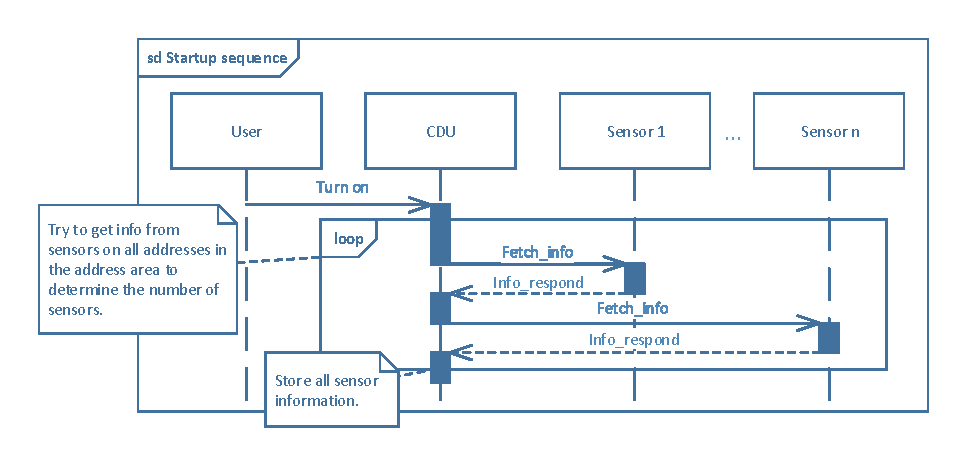
\includegraphics[width=.9\textwidth]{billeder/Startup_Sequence_SD}
\caption{Startup sequence}
\end{figure}
If there is no response from an address the CDU assumes there is no sensor on this address.

%Statemaskine for hver blok (nødvendig?)\\

\subsection{Normal Operation}
The goal of normal operation is to constantly acquire data from all sensors discovered in the startup sequence.

\begin{figure}[hbpt]
\centering
\includegraphics[width=.9\textwidth]{billeder/normal_operation_SD}
\caption{Normal operation}
\end{figure}

\subsection{Data extraction}
The goal of data extraction is to store all collected data on a PC so that it can be used i excel og similar.

\begin{figure}[hbpt]
\centering
\includegraphics[width=.6\textwidth]{billeder/data_extraction_sd}
\caption{Data extraction}
\end{figure}

\newpage

\section{Detailed block behaviour}
This section describes the overall behaviour of the two blocks in the system.\\
These statemachines are based upon the earlier behavioural architecture, but are more detailed.

\subsection{CDU}

\begin{figure}[hbpt]
\centering
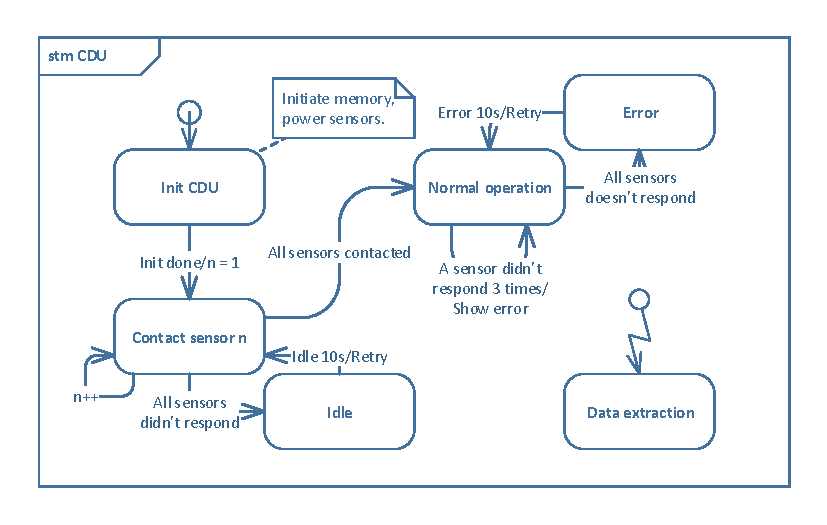
\includegraphics[width=.8\textwidth]{billeder/CDU_STM}
\caption{CDU statemachine}
\end{figure}
All errors must be logged in memory aswell.

\subsection{Sensor node}

\begin{figure}[hbpt]
\centering
\includegraphics[width=.8\textwidth]{billeder/sensor_node_STM}
\caption{Sensor node statemachine}
\end{figure}